
\chapter{模板使用方法}

对于一篇毕业论文,基于latex写作的时候,我们需要关注的就是如何插入图片、文献、表格、公式以及如何交叉引用。主要就是这几点,当然还有一些细节性的东西,作者会持续更新到 \href{https://www.jianshu.com/p/c9bb775fe0f4}{简书文章: CugTheis使用说明}  里面。

\subsection{插入图片}
\begin{figure} [htbp] 
	\centering
	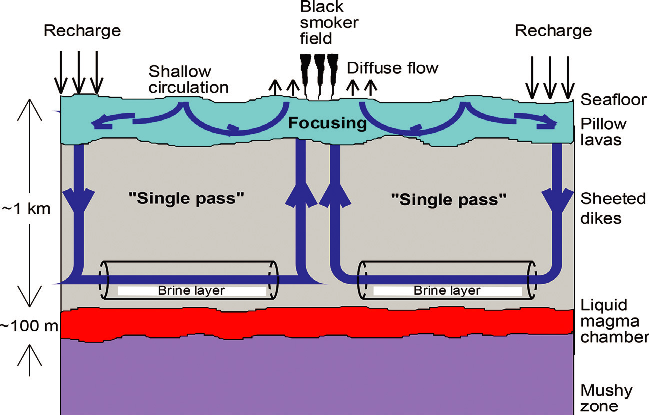
\includegraphics[width=\textwidth ]{SinglePassModel} 
	\caption[单通道模型]{Single Pass Model} 
	\fnote{海底热液循环系统示意图,包含了recharge区域和discharge区域。海水被岩浆热源加热后在深部发生 相分离,分离为密度较大的卤水(液相)和密度较小的蒸汽相,向上浮动。\textcolor{green}{这是一个但排列图}} 
	\label{fig:singlepassmodel} 
\end{figure} 

 \autoref{fig:singlepassmodel} 是一个单排列图\footnote{这是个脚注:注意这里的参考文献引用}
  \citep{andersen2017faulting}。每个图可根据实际意义命名一个label,方便后面进行交叉引用。
  caption设置是必须的,表示这个图的标题。如果此图有一段图注的话,使用fnote来设置。看 \autoref{fig:singlepassmodel} 的latex代码。为了生成图和表的索引,在图和表的caption前面也可以用方括号设置其shor-caption用于后面的图和表索引标题显示,比如  \autoref{fig:singlepassmodel} 的\textbf{单通道模型} 短标题。


\begin{figure} [htbp]
	\centering%
	\subcaptionbox{CUG彩色logo\label{fig:cug1} }  
	{
\includegraphics[height=0.23\textwidth]{CUG_Logo1} } 
	\hspace{0.01\textwidth} 
	\subcaptionbox{TAG热液系统结构图\label{fig:TAG} }  
	{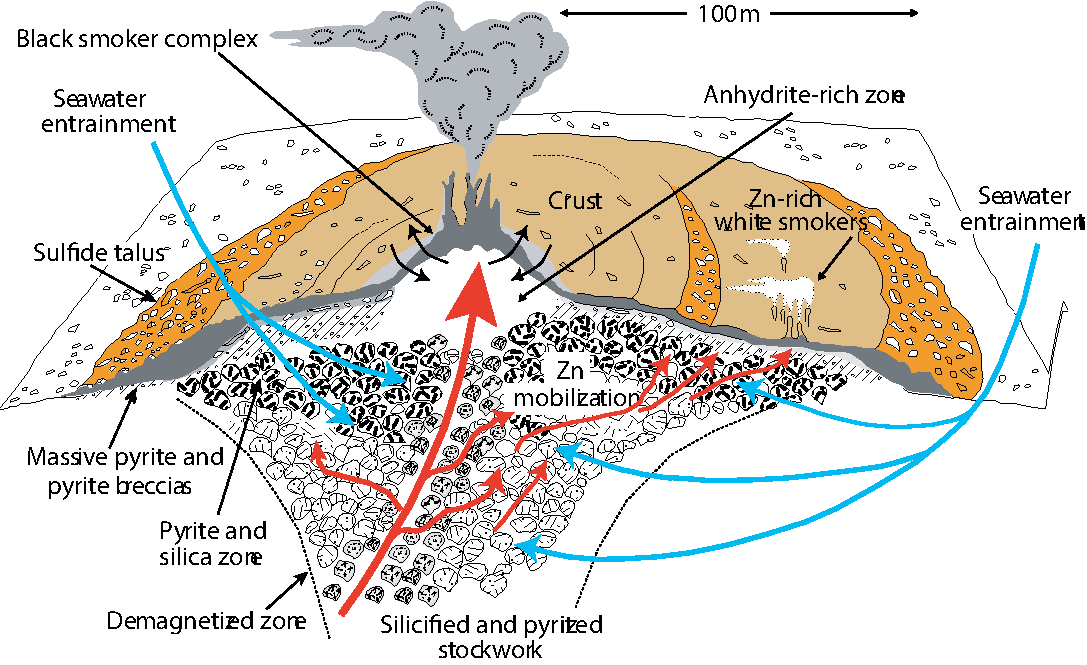
\includegraphics[height=0.23\textwidth]{TAG_structure_tivey} } 
		\hspace{0.01\textwidth} 
	\subcaptionbox{CUG黑白logo\label{fig:cug2} }  
	{
\includegraphics[height=0.23\textwidth]{CUG_Logo2} } 
	\caption{三列图示例} 
	\label{fig:figure_3col} 
\end{figure} 

\autoref{fig:figure_3col} 是一个三列子图示例,总图有编号和标题。每个子图也有相应的编号和标题,也可以交叉引用其中一个子图,比如 \autoref{fig:TAG} 表示位于MAR 的TAG热液系统的结构图。


\subsection{表格}

本模板支持三线表比如

\begin{table}[htbp]
	\centering
	\caption{数学符号和物理意义列表}
	\label{tab:symbols_values}
	\begin{tabular}{cccc}
		\toprule 
		数学符号 & 物理意义 & 典型取值 &单位 \\
		\midrule
		$\vec{g}$ & 重力加速度矢量 & 9.8 & $m/s^2$ \\
		$\rho_f$ & 水的密度 & 1.0 & $kg/m^3$ \\
		\bottomrule
	\end{tabular}
\end{table}

\autoref{tab:symbols_values} 是一个三线表,有其标题和label(用于交叉引用)。

\subsection{公式}

行内公式,这个是行内公式 $E=MC^2$,下面是个带编号的独立公式:

\begin{equation}
\left( {\phi {\rho _f}{c_{pf}} + \left( {1 - \phi } \right){\rho _r}{c_{pr}}} \right)\frac{{\partial T}}{{\partial t}} = \nabla  \cdot \left( {{K_r}\nabla T} \right) - {\rho _f}{c_{pf}}\vec v \cdot \nabla T + \frac{{{\mu _f}}}{k}{\vec v^2} - {\left( {\frac{{\partial \;ln\rho }}{{\partial \;lnT}}} \right)_p}\frac{{Dp}}{{Dt}}
\label{eq:EnergyConservation}
\end{equation}

这里引用公式,公式 \ref{eq:EnergyConservation} 表示了热液流体循环过程中的能量守恒。

\subsection{参考文献}
第一种引用方式:\cite{vehling2018implementation} 进行了相分离的数值模拟研究。
第二种引用方式:三维数值模拟目前仅限于单相流体\citep{coumou2008structure,coumou2006dynamics}。
这样的引用方式可能更易读一些,有可能地大要求以编号的形式显示,name只需要在main.tex里面把参考引用格式从{cugthesis-author-year}改为{cugthesis-numeric即可}